\documentclass[11pt,a4paper,oneside]{report}                    % Single-side

\usepackage[english,magyar]{babel}
\usepackage{amssymb}
\usepackage{enumerate}
\usepackage[thmmarks]{ntheorem}
\usepackage{graphicx}
\usepackage{color}
\usepackage[chapter]{minted}            % Objective-C és Swift kód színezéséért.
\usepackage{fancyhdr}
\usepackage{anysize}                    % Segítség az oldal marginjának beállításához.
\usepackage{sectsty}
\usepackage{setspace}                   % A csomag segítségével a táblázatok, ábrák, lábjegyzetek 1-es sorközzel maradhatnak.
\usepackage{newfloat}
\usepackage[table,xcdraw]{xcolor}       % Színes táblázatokért.
\usepackage{hyperref}                   % A PDF-ben levő linkek megjelnése és működése érdekében.
\usepackage[hang]{caption}
\usepackage{subcaption}                 % Egymás mellett lévő képekért
\usepackage{hyphenat}                   % Kötőjelet tartalmazó szavak elválasztásához.
\usepackage{pdfpages}                   % Meglévő .pdf fájlok beillesztéséhez.
\usepackage[export]{adjustbox}          % textwidth-nél szélesebb képek középre igazításához
\usepackage{tabularx}                   % dinamikus szélességű táblázatért
\usepackage[fleqn]{amsmath}             
\usepackage{tcolorbox}                  % http://tex.stackexchange.com/questions/305387/adding-a-caption-to-a-tcolorbox-tcblisting
\usepackage[autostyle]{csquotes}        % Magyar idézőjelekért.

%--------------------------------------------------------------------------------------
% Main variables
%--------------------------------------------------------------------------------------
\newcommand{\vikszerzo}{Név}
\newcommand{\vikkonzulens}{Konzulens}
\newcommand{\vikcim}{Dolgozat címe}
\newcommand{\viktanszek}{Automatizálási és Alkalmazott Informatikai Tanszék}
\newcommand{\vikdoktipus}{Szakdolgozat/Diplomaterv}
\newcommand{\vikdepartmentr}{}

%--------------------------------------------------------------------------------------
% Page layout setup
%--------------------------------------------------------------------------------------
\pagestyle{plain}
\setlength{\parindent}{12pt}                 % magyar nyelvű dokumentumokban jellemző
\setlength{\parskip}{0pt}                    % magyar nyelvű dokumentumokban jellemző

\marginsize{35mm}{25mm}{15mm}{15mm}          % anysize package
\sectionfont{\large\upshape\bfseries}
\setcounter{secnumdepth}{2}
\singlespacing
\frenchspacing

\hyphenation{iOS}
\hyphenation{macOS}

%--------------------------------------------------------------------------------------
% Setup hyperref package
%--------------------------------------------------------------------------------------
\hypersetup{
    bookmarksnumbered=true,     % put section numbers in bookmarks
    unicode=false,              % Unicode encoded pdf strings
    pdftitle={\vikcim},         % text for PDF Title field
    pdfauthor={\vikszerzo},     % text for PDF Author field
    pdfsubject={\vikdoktipus},  % text for PDF Subject field
    pdfcreator={\vikszerzo},    % text for PDF Creator field
    pdfproducer={LaTeX},        % text for PDF Producer field
    pdfkeywords={keywords},     % text for PDF Keywords field
    pdfnewwindow=true,          % make links that open another PDF file start a new window
    colorlinks=true,            % colored links
    linkcolor=black,            % color of links
    citecolor=black,            % color of citation links
    filecolor=black,            % color of file links
    urlcolor=black              % color of URL links
}

%--------------------------------------------------------------------------------------
% Set up listings
%--------------------------------------------------------------------------------------
\tcbuselibrary{listings,minted,skins,breakable}
\renewcommand*\thelstnumber{\ifnum\value{lstnumber}<10 0\fi\the\value{lstnumber}}
\renewcommand{\lstlistingname}{kódrészlet}
\renewcommand{\listoflistingscaption}{Kódrészletek jegyzéke}

\makeatletter
\renewcommand\fnum@lstlisting{%
  \ifx\lst@@caption\@empty\else\thelstlisting~\fi%
  \lstlistingname}%
\tcbset{
  new/blend into/revlistings/.style={use counter*=lstlisting,list inside=lol,/tcb/code={\appto\tcb@new@colopt{,before title={\tcb@blend@beforetitle{\textbf{\thetcbcounter.~\lstlistingname}}}}}},%
}
\makeatother

\makeatletter
\AtBeginDocument{\let\c@listing\c@lstlisting}
\makeatother

\AtBeginDocument{%
  \newtcblisting[blend into=revlistings]{code}[3]{%
    breakable,
    colback=codebg,
    colframe=black!40,
    enhanced,
    listing engine=minted,
    listing only,
    left=5mm,
    overlay={\begin{tcbclipinterior}\fill[black!25] (frame.south west)
      rectangle ([xshift=5mm]frame.north west);\end{tcbclipinterior}},
    listing remove caption=false,
    minted style=colorful,
    minted language=#1,
    minted options={linenos=true,numbersep=3mm,texcl=true,breaklines=true,autogobble=true},
    coltitle=black,
    attach boxed title to bottom center={yshift=-10pt},
    boxed title style={colback=white, sharp corners, boxrule=-1pt},
    #2
  }
}
\definecolor{codebg}{rgb}{0.95,0.95,0.95}

%--------------------------------------------------------------------------------------
% Setup tabularx package
%--------------------------------------------------------------------------------------
\def\tabularxcolumn#1{m{#1}}  % vertically centered cells

%--------------------------------------------------------------------------------------
% Some new commands and declarations
%--------------------------------------------------------------------------------------
\newcommand{\chapref}[1]{\ref{chap:#1}}
\newcommand{\chaparef}[1]{\aref{chap:#1}}
\newcommand{\chapAref}[1]{\Aref{chap:#1}}

\newcommand{\figref}[1]{\ref{fig:#1}.}
\newcommand{\figaref}[1]{\aref{fig:#1}.}
\newcommand{\figAref}[1]{\Aref{fig:#1}.}

\newcommand{\listref}[1]{\ref{lst:#1}. kódrészlet}
\newcommand{\listaref}[1]{\aref{lst:#1}. kódrészlet}
\newcommand{\listAref}[1]{\Aref{lst:#1}. kódrészlet}

\newcommand{\sectref}[1]{\ref{sect:#1}}
\newcommand{\sectaref}[1]{\aref{sect:#1}}
\newcommand{\sectAref}[1]{\Aref{sect:#1}}

\newcommand{\tabref}[1]{\ref{tab:#1}.}
\newcommand{\tabaref}[1]{\aref{tab:#1}.}
\newcommand{\tabAref}[1]{\Aref{tab:#1}.}

\newcommand{\boldurl}[1]{\href{#1}{\textbf{#1}}}

\author{\vikszerzo}

%--------------------------------------------------------------------------------------
%   Setup captions
%--------------------------------------------------------------------------------------
\captionsetup{
justification=justified,
width=.75\textwidth,
aboveskip=10pt}

\renewcommand{\captionlabelfont}{\small\bf}
\renewcommand{\captionfont}{\footnotesize\it}

%--------------------------------------------------------------------------------------
%   Setup csquotes
%--------------------------------------------------------------------------------------
\DeclareQuoteStyle{magyar}
{\quotedblbase}
{\textquotedblright}
[.05em]
{\guillemotright}
{\guillemotleft}

%--------------------------------------------------------------------------------------
% Table of contents and the main text
%--------------------------------------------------------------------------------------
\begin{document}
\pagenumbering{arabic}
\onehalfspacing

% Feladatkiírás hozzáfüzése .pdf fájlból
%\setcounter{secnumdepth}{-1}
%\includepdf[pages=-,addtotoc={1,chapter,0,Feladatkiírás,sect:feladatkiiras}]{feladatkiiras.pdf}
%\setcounter{secnumdepth}{2}

% A dolgozat címe
%--------------------------------------------------------------------------------------
%	The title page
%--------------------------------------------------------------------------------------
\begin{titlepage}
  \thispagestyle{empty}
  \begin{center}
    
\includegraphics[width=60mm,keepaspectratio]{figures/BMElogo.png}\\
    \vspace{0.3cm}
    \textbf{Budapesti Műszaki és Gazdaságtudományi Egyetem}\\
    \textmd{Villamosmérnöki és Informatikai Kar}\\
    \textmd{\viktanszek}\\[5cm]
    
    \vspace{0.4cm}
    {\huge \bfseries \vikcim}\\[0.8cm]
    \vspace{0.5cm}
    \textsc{\Large \vikdoktipus}\\[4cm]
    
    \begin{tabular}{cc}
      \makebox[7cm]{\emph{Készítette}} & \makebox[7cm]{\emph{Konzulens}} \\
      \makebox[7cm]{\vikszerzo} & \makebox[7cm]{\vikkonzulens}
    \end{tabular}
    
    \vfill
    {\large \today}
  \end{center}
\end{titlepage}




% Tartalomjegyzék
\tableofcontents\vfill

% Nyilatkozat
%--------------------------------------------------------------------------------------
% Nyilatkozat
%--------------------------------------------------------------------------------------
\begin{center}
\large
\textbf{HALLGATÓI NYILATKOZAT}\\
\end{center}

Alulírott \emph{\vikszerzo}, szigorló hallgató kijelentem, hogy ezt a diplomatervet meg nem engedett segítség nélkül, saját magam készítettem, csak a megadott forrásokat (szakirodalom, eszközök stb.) használtam fel. Minden olyan részt, melyet szó szerint, vagy azonos értelemben, de átfogalmazva más forrásból átvettem, egyértelműen, a forrás megadásával megjelöltem.

Hozzájárulok, hogy a jelen munkám alapadatait (szerző(k), cím, angol és magyar nyelvű tartalmi kivonat, készítés éve, konzulens(ek) neve) a BME VIK nyilvánosan hozzáférhető elektronikus formában, a munka teljes szövegét pedig az egyetem belső hálózatán keresztül (vagy autentikált felhasználók számára) közzétegye. Kijelentem, hogy a benyújtott munka és annak elektronikus verziója megegyezik. Dékáni engedéllyel titkosított diplomatervek esetén a dolgozat szövege csak 3 év eltelte után válik hozzáférhetővé.

\begin{flushleft}
\vspace*{1cm}
Budapest, \today
\end{flushleft}

\begin{flushright}
 \vspace*{1cm}
 \makebox[7cm]{\rule{6cm}{.4pt}}\\
 \makebox[7cm]{\emph{\vikszerzo}}\\
 \makebox[7cm]{hallgató}
\end{flushright}
\thispagestyle{empty}

\vfill
\clearpage
\thispagestyle{empty} % an empty page


% Kivonat - Abstract
%----------------------------------------------------------------------------
% Abstract in Hungarian
%----------------------------------------------------------------------------
\chapter*{Kivonat}\addcontentsline{toc}{chapter}{Kivonat}

\vfill

%----------------------------------------------------------------------------
% Abstract in English
%----------------------------------------------------------------------------
\begin{otherlanguage}{english}
\chapter*{Abstract}\addcontentsline{toc}{chapter}{Abstract}

\end{otherlanguage}


% Bevezetés
%----------------------------------------------------------------------------
\chapter{Bevezető}
%----------------------------------------------------------------------------
Bevezető bevezetője. Árvíztűrő tükörfúrógép.

\section*{Célkitűzés}\addcontentsline{toc}{section}{Célkitűzés}
Új számozatlan alfejezet létrehozása (és a tartalomjegyzékhez adása). 

Felsorolás:
\begin{itemize}
  \item elem,
  \item másik elem,
  \item utolsó elem.
\end{itemize}

\section*{Témaválasztás indoklása}\addcontentsline{toc}{section}{Témaválasztás indoklása}

\section*{A dolgozat felépítése}\addcontentsline{toc}{section}{A dolgozat felépítése}


% 1. fejezet - Az Objective-C és Swift nyelv rövid összehasonlítása
\chapter{Az \textit{Objective-C} és \textit{Swift} nyelv rövid összehasonlítása}

Szinten mindenhez lehet opcionálisan \textit{label}t hozzáadni, majd utána ennek segítségével hivatkozni rá. Ezen felül a LaTeX még automatikusan tud rakni a szám elé a/A/az/Az névelőket. Például \sectaref{objc-c-short-history} alfejezetben az Objective-C rövid története kerül bemutatásra. \sectAref{objc-c-short-history} alfejezet némiképp hiányos.

\section{Az \textit{Objective-C} nyelv rövid története}
\label{sect:objc-c-short-history}
Hivatkozhatunk könyvekre, cikkekre vagy akár weboldalakra is.\cite{UncleBob} Kép berakására ezt a \enquote{snippetet} ajánlom. \figAref{git-flow} képen a git-flow workflow látható.

\begin{figure}[H]
  \centering
  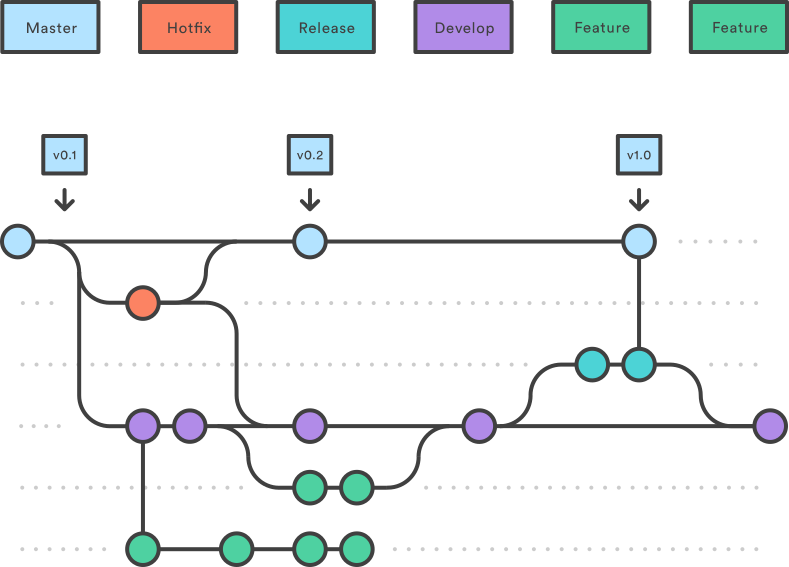
\includegraphics[width=0.7\textwidth, keepaspectratio]{figures/example_image.png}
  \caption{Git-flow workflow}
  \label{fig:git-flow}
\end{figure}

Mindenféle kódot is berakhatunk, nem mindig tökéletes eredménnyel.

\begin{otherlanguage}{english}
  \begin{code}{swift}{title={A kódrészlet  \enquote{címe}}, label={lst:drop-proposal}}
func collectionView(_ collectionView: UICollectionView, dropSessionDidUpdate session: UIDropSession, withDestinationIndexPath destinationIndexPath: IndexPath?) -> UICollectionViewDropProposal {
  if collectionView.hasActiveDrag {
    return UICollectionViewDropProposal(operation: .move, intent: .insertAtDestinationIndexPath)
  } else {
    return UICollectionViewDropProposal(operation: .copy, intent: .insertAtDestinationIndexPath)
  }
}  
  \end{code}
\end{otherlanguage}

Táblázatokhoz ajánlom használni \href{https://www.tablesgenerator.com}{ezt} az oldalt:

\begin{table}[H]
  \begin{tabular}{|c|c|}
    \hline
    név        & szín       \\ \hline
    alma       & piros/zöld \\ \hline
    körte      & sárga      \\ \hline
    cseresznye & piros      \\ \hline
  \end{tabular}
\end{table}

Hosszú URLeknél, előfordulhat hogy a \verb=\url{}=\cite{LongUrlExample1} parancs nem tördeli jól az URL-eket (túlfolyik a margón). Ennek kikerülésére használható a \verb=\boldurl{}=\cite{LongUrlExample2} parancs.

%----------------------------------------------------------------------------
\chapter{Összefoglalás}
%----------------------------------------------------------------------------



% Ábrák jegyzéke
\listoffigures\addcontentsline{toc}{chapter}{Ábrák jegyzéke}
% Kódrészletek jegyzéke
\listoflistings\addcontentsline{toc}{chapter}{Kódrészletek jegyzéke}
% Táblázatok jegyzéke
\listoftables\addcontentsline{toc}{chapter}{Táblázatok jegyzéke}

% Irodalomjegyzék
\bibliography{mybib}
\bibliographystyle{plain}
\addcontentsline{toc}{chapter}{Irodalomjegyzék}

\end{document}
